\documentclass[aspectratio=169,11pt]{beamer}
% Compile with pdflatex. Style: Computer Modern, white background, amber labels, blue citations.
\usetheme{default}
\usepackage[T1]{fontenc}
\usepackage{lmodern}
\usepackage{booktabs,array,xcolor,tikz,amsmath}
\usetikzlibrary{arrows.meta,positioning,calc}
\setbeamertemplate{navigation symbols}{}
\setbeamertemplate{footline}{\hfill{\scriptsize\color{muted}\insertframenumber\,/\,\inserttotalframenumber}\hspace{0.45cm}\vspace{0.25cm}}
\setbeamertemplate{itemize items}[triangle]
\setbeamertemplate{frametitle}{\vspace{0.55cm}\textbf{\large\insertframetitle}\par}
\usefonttheme{serif}
\definecolor{ink}{HTML}{1F1F1F}
\definecolor{muted}{HTML}{6B6B6B}
\definecolor{amber}{HTML}{B07D0E}
\definecolor{teal}{HTML}{1F6F5F}
\definecolor{cite}{HTML}{2A5DB0}
\setbeamercolor{normal text}{fg=ink}
\setbeamercolor{frametitle}{fg=ink}
\setbeamercolor{title}{fg=ink}
\setbeamercolor{itemize item}{fg=teal}
\setbeamersize{text margin left=1.1cm,text margin right=1.1cm}
\newcommand{\lab}[1]{\textcolor{amber}{\textbf{#1}}}
\newcommand{\muted}[1]{{\color{muted}#1}}
\newcommand{\cit}[1]{{\color{cite}\small(#1)}}
\newcolumntype{L}[1]{>{\raggedright\arraybackslash}p{#1}}
\renewcommand{\arraystretch}{1.3}\setlength{\tabcolsep}{4pt}

\title{\textbf{The Anatomy of the Principal Effect}}
\subtitle{Teachers, classrooms, and families under mandatory turnover}
\author{}
\date{\muted{Paper idea for discussion. October 2026}}

\begin{document}

\begin{frame}[plain]
\titlepage
\end{frame}

%% 1. The question
\begin{frame}[plain]
\vspace{1.3cm}
\begin{center}
{\LARGE\textbf{What does a school leader change,}\\[0.2em]\textbf{and how far does it reach?}}
\end{center}
\vspace{0.9cm}
\begin{center}
\begin{minipage}{0.78\textwidth}
Principal value added on test scores is well documented. The process behind it, how leadership affects teachers, classrooms, and families, is not.
\end{minipage}
\end{center}
\end{frame}

%% 2. What we know
\begin{frame}[label=know]{What we know}
\vspace{0.1cm}
\small
\begin{tabular}{@{}L{3.1cm}L{9.9cm}@{}}
\lab{Magnitude} & One SD of principal quality: 0.05 to 0.10 SD of achievement \cit{Branch, Hanushek, and Rivkin, 2012; B\"ohlmark, Gr\"onqvist, and Vlachos, 2016}; 0.03 in math and 0.01 in reading once time-varying school shocks are removed \cit{Bartanen, Husain, and Liebowitz, 2024}. \\[0.3em]
\lab{Turnover} & A change of principal lowers achievement by 0.03 SD and raises teacher turnover \cit{Bartanen, Grissom, and Rogers, 2019}. \\[0.3em]
\lab{Mechanism} & Personnel: effective principals retain high-value-added teachers and dismiss low-rated ones \cit{Grissom and Bartanen, 2019; Mu\~noz and Prem, 2024}; they change the composition of the staff \cit{Bartanen and Grissom, 2023}. \\[0.3em]
\lab{Open} & Effects on the same teachers' practice and wellbeing, on classrooms, and on families, under exogenous turnover. \\
\end{tabular}
\vspace{0.1cm}
\hfill\hyperlink{recent}{\beamerbutton{Recent work}}
\end{frame}

%% 3. Outcomes
\begin{frame}{Outcomes}
\vspace{0.1cm}
\small
\begin{tabular}{@{}L{3.1cm}L{9.9cm}@{}}
\lab{Teachers} & Classroom practice, collaboration, training, self-efficacy, wellbeing. \\[0.4em]
\lab{Classrooms} & Allocation of teachers and support hours across groups, discipline, safety. \\[0.4em]
\lab{Families} & Involvement, satisfaction with teachers and school, perceived quality. \\[0.4em]
\lab{Pupils} & Engagement, perceptions of the school, standardized achievement by subject. \\
\end{tabular}
\vspace{0.6cm}

All four are observed for every school and year. The first three are outcomes in their own right and the channels to the fourth.
\end{frame}

%% 4. Causal map
\begin{frame}{Causal map}
\vspace{0.2cm}
\begin{center}
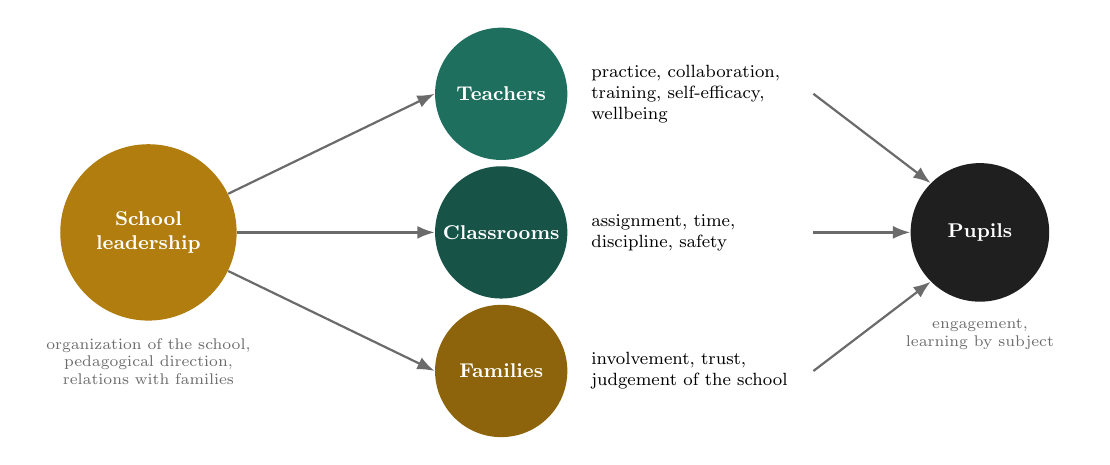
\begin{tikzpicture}[scale=0.8,every node/.style={font=\small,transform shape},
  circ/.style={circle,draw=none,text=white,align=center,font=\small\bfseries,minimum size=2.1cm,inner sep=1pt},
  lbl/.style={align=left,font=\footnotesize,text width=3.4cm},
  arr/.style={-{Latex[length=2.2mm]},line width=0.8pt,draw=muted}
]
\node[circ,fill=amber,minimum size=2.8cm] (lead) at (0,0) {School\\leadership};
\node[below=0.15cm of lead,font=\scriptsize,text=muted,align=center,text width=3.6cm] {organization of the school,\\pedagogical direction,\\relations with families};
\node[circ,fill=teal] (teach) at (5.6,2.2) {Teachers};
\node[circ,fill=teal!75!black] (clim) at (5.6,0) {Classrooms};
\node[circ,fill=amber!80!black] (fam) at (5.6,-2.2) {Families};
\node[lbl,right=0.25cm of teach] (t1) {practice, collaboration,\\training, self-efficacy,\\wellbeing};
\node[lbl,right=0.25cm of clim] (t2) {assignment, time,\\discipline, safety};
\node[lbl,right=0.25cm of fam] (t3) {involvement, trust,\\judgement of the school};
\node[circ,fill=ink,minimum size=2.2cm] (learn) at (13.2,0) {Pupils};
\node[below=0.15cm of learn,font=\scriptsize,text=muted,align=center,text width=3cm] {engagement,\\learning by subject};
\draw[arr] (lead) -- (teach.west);
\draw[arr] (lead) -- (clim.west);
\draw[arr] (lead) -- (fam.west);
\draw[arr] (t1.east) -- (learn.north west);
\draw[arr] (t2.east) -- (learn.west);
\draw[arr] (t3.east) -- (learn.south west);
\end{tikzpicture}
\end{center}
\vspace{0.05cm}
\muted{\small Exogenous variation enters at the leadership node.}
\end{frame}

%% 5. Setting
\begin{frame}{Setting: Madrid public primary schools}
\vspace{0.1cm}
\small
\begin{tabular}{@{}L{3.1cm}L{9.9cm}@{}}
\lab{Principals} & Teachers selected from the staff for four-year terms. They do not hire, dismiss, set pay, or set the curriculum. \\[0.4em]
\lab{Implication} & A change of principal changes leadership and organization on a fixed staff. The personnel channel is shut by design. \\[0.4em]
\lab{Mandatory exits} & Compulsory retirement at 65. At most two renewals: twelve years in office. Both dates are known years in advance. \\[0.4em]
\lab{Successors} & Come from the same staff. Observed as classroom teachers in the year before appointment. \\
\end{tabular}
\end{frame}

%% 6. Mandatory exits
\begin{frame}{Identification: mandatory exits}
\vspace{0.05cm}
\begin{center}
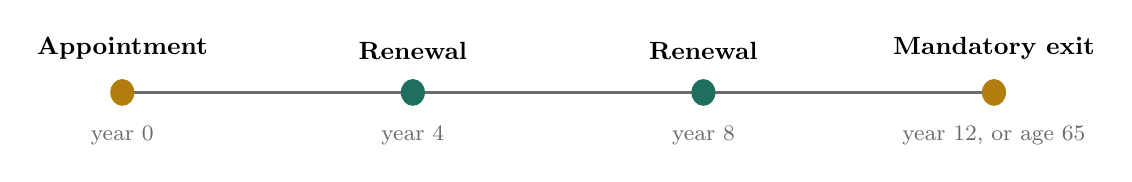
\begin{tikzpicture}[x=0.9cm,y=1cm]
\draw[muted,line width=0.8pt] (0,0) -- (12.4,0);
\foreach \x/\lbl/\sub/\col in {0/Appointment/{year 0}/amber, 4.1/Renewal/{year 4}/teal, 8.2/Renewal/{year 8}/teal, 12.3/Mandatory exit/{year 12, or age 65}/amber}{
  \fill[\col] (\x,0) circle (0.17);
  \node[above=0.3cm,font=\small\bfseries] at (\x,0) {\lbl};
  \node[below=0.3cm,font=\footnotesize,text=muted] at (\x,0) {\sub};
}
\end{tikzpicture}
\end{center}
\vspace{-0.2cm}
\small
\begin{tabular}{@{}L{3.1cm}L{9.9cm}@{}}
\lab{Treatment} & A principal exit forced by the age or tenure rule in 2016, 2017, or 2018. \\[0.3em]
\lab{Control} & Schools whose principal has not yet reached either limit. \\[0.3em]
\lab{Assumption} & The date of a mandatory exit is unrelated to contemporaneous school shocks. Testable on pre-trends. \\[0.3em]
\lab{Excluded} & Voluntary exits (resignation, non-renewal). Estimated separately as the selection benchmark. \\
\end{tabular}
\end{frame}

%% 7. Event study
\begin{frame}{Event study}
\vspace{0.1cm}
\small
$\tau_s$: year of the mandatory exit in school $s$. $i$: a teacher, classroom, pupil, or parent.
\begin{equation*}
Y_{ist}=\alpha_s+\lambda_t+\sum_{k\neq -1}\beta_k\,\mathbf{1}[\,t-\tau_s=k\,]+\varepsilon_{ist}
\end{equation*}
\vspace{0.1cm}
\begin{tabular}{@{}L{2.6cm}L{10.4cm}@{}}
\lab{$\beta_k$, $k\ge0$} & Effect $k$ years after the exit, relative to the year before. \\[0.3em]
\lab{$\beta_k$, $k<0$} & Pre-trend test: zero if the exit date is exogenous. \\[0.3em]
\lab{Inference} & Not-yet-treated schools as controls; staggered-robust estimator; clustered by school. \\
\end{tabular}
\end{frame}

%% 8. IV
\begin{frame}{Effect of a change of principal}
\vspace{0.1cm}
\small
$Z_{st}=\mathbf{1}[t\ge\tau_s]$: the rule binds. $D_{st}=\mathbf{1}[\text{new principal}]$: the realized change.
\begin{align*}
D_{st}&=\pi Z_{st}+\alpha_s+\lambda_t+u_{st} \\
Y_{ist}&=\beta\,\widehat{D}_{st}+\alpha_s+\lambda_t+\varepsilon_{ist}
\end{align*}
\vspace{0.1cm}
\begin{tabular}{@{}L{2.6cm}L{10.4cm}@{}}
\lab{$\beta$} & Effect of a new principal where the rule forced the change. \\[0.3em]
\lab{$\pi$} & Equal to one for retirement. Below one for the tenure limit: the incumbent may be re-selected. \\[0.3em]
\lab{Within unit} & Teacher fixed effects for the same teacher under two principals. Lagged score for the same pupil in grades 3 and 6. \\
\end{tabular}
\end{frame}

%% 9. Variance
\begin{frame}{Variance of principal effects}
\vspace{0.1cm}
\small
$Y_{st}=\mu_s+\theta_{p(s,t)}+e_{st}$, where $\theta$ is the effect of the principal in office.
\begin{equation*}
\mathrm{Var}\big(\Delta Y_{st}\mid Z_{st}=1\big)-\mathrm{Var}\big(\Delta Y_{st}\mid Z_{st}=0\big)=2\,\sigma^2_{\theta}
\end{equation*}
\vspace{0.1cm}
\begin{tabular}{@{}L{2.6cm}L{10.4cm}@{}}
\lab{$\sigma^2_\theta$} & Dispersion of principal effects on each outcome, without ranking principals \cit{Jones and Olken, 2005}. \\[0.3em]
\lab{Assumption} & $e_{st}$ independent of $Z_{st}$. Same pre-trend test. \\[0.3em]
\lab{Use} & Separates ``principals do not matter'' from ``effects cancel on average''. \\
\end{tabular}
\end{frame}

%% 10. Heterogeneity
\begin{frame}{Heterogeneity by pre-determined characteristics}
\vspace{0.1cm}
\small
\begin{equation*}
Y_{ist}=\alpha_s+\lambda_t+\beta\,D_{st}+\delta\,D_{st}\times W_s+\varepsilon_{ist}
\end{equation*}
\vspace{0.1cm}
\begin{tabular}{@{}L{2.6cm}L{10.4cm}@{}}
\lab{$W_s$} & Measured before appointment: the successor's practices and wellbeing as a teacher in $\tau_s-1$; the selection committee's score of their project; the staff's rating of the outgoing principal in $\tau_s-1$. \\[0.3em]
\lab{$\delta$} & Variation of the effect with who leaves and who arrives. \\[0.3em]
\lab{Check} & $W_s$ uncorrelated with pre-trends. \\
\end{tabular}
\end{frame}

%% 11. Timing
\begin{frame}{Outcomes and expected timing}
\vspace{-0.05cm}
\footnotesize\begin{tabular}{@{}L{2.0cm}L{5.9cm}L{3.3cm}L{1.5cm}@{}}
\toprule
\textbf{Domain} & \textbf{Outcome} & \textbf{Source} & \textbf{When} \\
\midrule
\lab{Classrooms} & Assignment of teachers and support hours across groups & Timetables, class composition & Year 1 \\
\lab{Classrooms} & Discipline and climate & Pupil and teacher reports & Years 1--2 \\
\lab{Families} & Involvement, trust, judgement of the school & Parent survey & Years 1--2 \\
\lab{Teachers} & Self-efficacy, wellbeing, collaboration, training & Teacher survey & Years 1--2 \\
\lab{Teachers} & Classroom practice, within teacher & Teacher survey & Years 2--3 \\
\lab{Pupils} & Engagement and achievement by subject & Pupil survey, tests & Last \\
\bottomrule
\end{tabular}
\vspace{0.0cm}

\muted{\footnotesize Pre-registered indices by domain.}
\end{frame}

%% 12. Data
\begin{frame}{Data}
\vspace{0.1cm}
\small
\begin{tabular}{@{}L{3.1cm}L{9.9cm}@{}}
\lab{In hand} & Universe of Madrid public primary schools, 2015 to 2018. Principal questionnaire. Teacher questionnaire: practices, wellbeing, training. Timetables. All pupils by classroom: scores by subject, perceptions. All parents by classroom: involvement, satisfaction. \\[0.4em]
\lab{To collect} & Principal appointments, renewals, and exits with cause (BOCM). Committee score of each project. Teacher assignment lists. School plans from archived websites. Public school-level results from 2022. \\
\end{tabular}
\end{frame}

%% 13. Open questions
\begin{frame}{Open questions}
\vspace{0.3cm}
\begin{itemize}\setlength{\itemsep}{0.9em}
\item \textbf{Which outcomes first.} Which domains should respond in the first year of a new principal.
\item \textbf{Data requirements.} Stable teacher identifier across years; principal's age and years in office; survey items rating the principal.
\item \textbf{Sample.} Number of mandatory exits in 2015 to 2018; access to appointment records and later years.
\end{itemize}
\end{frame}

%% References
\begin{frame}[allowframebreaks]{References}
\footnotesize
Bartanen, B., and J.~A. Grissom. 2023. ``School Principal Race, Teacher Racial Diversity, and Student Achievement.'' \textit{Journal of Human Resources} 58(2): 666--712.\\[0.35em]
Bartanen, B., J.~A. Grissom, and L.~Rogers. 2019. ``The Impacts of Principal Turnover.'' \textit{Educational Evaluation and Policy Analysis} 41(3): 350--374.\\[0.35em]
Bartanen, B., A.~N. Husain, and D.~D. Liebowitz. 2024. ``Rethinking Principal Effects on Student Outcomes.'' \textit{Journal of Public Economics} 234.\\[0.35em]
B\"ohlmark, A., E.~Gr\"onqvist, and J.~Vlachos. 2016. ``The Headmaster Ritual: The Importance of Management for School Outcomes.'' \textit{Scandinavian Journal of Economics} 118(4): 912--940.\\[0.35em]
Branch, G.~F., E.~A. Hanushek, and S.~G. Rivkin. 2012. ``Estimating the Effect of Leaders on Public Sector Productivity: The Case of School Principals.'' NBER Working Paper 17803.\\[0.35em]
Fenizia, A. 2022. ``Managers and Productivity in the Public Sector.'' \textit{Econometrica} 90(3): 1063--1084.\\[0.35em]
Grissom, J.~A., and B.~Bartanen. 2019. ``Strategic Retention: Principal Effectiveness and Teacher Turnover in Multiple-Measure Teacher Evaluation Systems.'' \textit{American Educational Research Journal} 56(2): 514--555.\\[0.35em]
Hanushek, E.~A., A.~Morgan, S.~G. Rivkin, J.~C. Schiman, A.~Shakeel, and L.~Sartain. 2024. ``The Lasting Impacts of Middle School Principals.'' NBER Working Paper 32642.\\[0.35em]
Jones, B.~F., and B.~A. Olken. 2005. ``Do Leaders Matter? National Leadership and Growth Since World War II.'' \textit{Quarterly Journal of Economics} 120(3): 835--864.\\[0.35em]
Lavy, V., A.~Boiko, and G.~Rachkovski. 2023. ``Effects and Mechanisms of CEOs Quality in Public Education.'' \textit{Economic Journal}.\\[0.35em]
Lemos, R., K.~Muralidharan, and D.~Scur. 2024. ``Personnel Management and School Productivity: Evidence from India.'' \textit{Economic Journal} 134.\\[0.35em]
Miller, A. 2013. ``Principal Turnover and Student Achievement.'' \textit{Economics of Education Review} 36: 60--72.\\[0.35em]
Mu\~noz, P., and M.~Prem. 2024. ``Managers' Productivity and Recruitment in the Public Sector: The Case of School Principals.'' \textit{American Economic Journal: Economic Policy} 16(4): 223--253.\\[0.35em]
Rahaman, A., and C.~Koedel. 2026. ``Principal Effects on Teacher Working Conditions.'' CALDER Working Paper 335.\\[0.35em]
Tsao, C. 2024. ``Managers in Public Schools.'' Working paper, Princeton University.
\end{frame}

%% Appendix
\begin{frame}[label=recent]{Appendix: recent work on school and public-sector leaders}
\vspace{-0.1cm}
\scriptsize
\renewcommand{\arraystretch}{1.0}
\begin{tabular}{@{}L{8.3cm}L{3.6cm}L{1.0cm}@{}}
\toprule
\textbf{Title} & \textbf{Journal} & \textbf{Year} \\
\midrule
Principal effects on teacher working conditions (Rahaman and Koedel) & CALDER WP & 2026 \\
Rethinking principal effects on student outcomes & J. Public Economics & 2024 \\
Managers' productivity and recruitment in the public sector: the case of school principals & AEJ: Economic Policy & 2024 \\
Personnel management and school productivity: evidence from India & Economic Journal & 2024 \\
The lasting impacts of middle school principals & NBER WP & 2024 \\
Managers in public schools (Tsao) & Princeton JMP & 2024 \\
Effects and mechanisms of CEOs quality in public education & Economic Journal & 2023 \\
School principal race, teacher racial diversity, and student achievement & J. Human Resources & 2023 \\
Managers and productivity in the public sector & Econometrica & 2022 \\
\bottomrule
\end{tabular}
\vspace{0.15cm}

\muted{\scriptsize Tsao: event studies of principal moves and retirements, Kentucky and Texas; effects on scores, absenteeism, teacher retention. Rahaman and Koedel: variance of principal effects on 20 teacher-reported working conditions, Illinois.}

\hfill\hyperlink{know}{\beamerreturnbutton{Back}}
\end{frame}

\end{document}
